\subsection{Functions of Two or Three Variables}

\BEN
% ~~~~~~~~~~~~~~~~~~~~~~~~~~~~~~~~~~~~~~~~~~~~~~~~~~~~~~~~~
%DOMAIN AND RANGE PROBLEMS
\item 
\begin{enumerate}
% -  -  -  -  -  -  -  -  -  -  -  -  -  -  -  -  -  -  -  -  -  -  -  -  -  -  -  -  -  -  
% PART A
\item The function is not defined when the denominator is zero, or when the argument of the square root is negative. Either $x$ and $y$ are greater than 1, or less than -1. The domain, $D$, is therefore
\begin{align*}D = \{(x,y)|x > 1, y > 1; \text{ and } x < -1, y < -1\}. \end{align*}
The function can't be zero, and cannot be negative, because the square root will always yield a positive number. The range is $f > 0$.  
\begin{figure}[!htbp]
  \begin{center}
    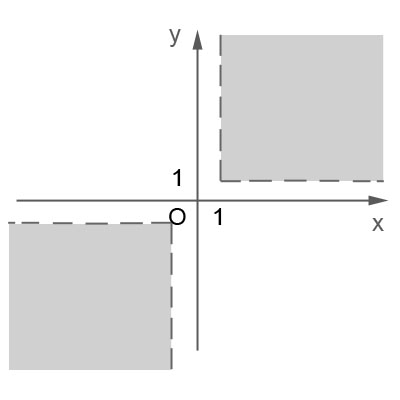
\includegraphics[width=0.4\textwidth]{Img1A.jpg}
  \end{center}
\end{figure}
% -  -  -  -  -  -  -  -  -  -  -  -  -  -  -  -  -  -  -  -  -  -  -  -  -  -  -  -  -  -  
% PART B
\item The function is not defined when the denominator is zero, so we require that $yx^2+xy^2\ne0$, or $xy(x+y)\ne0$. This implies that the function is not defined along the lines $x=0$, $y=0$, and $y=-x$. Moreover, the numerator has a square root. The argument must be non-negative, and so we also have the restriction that $y\ge-1$. The domain can therefore be expressed as $D=\{(x,y)| y\ge -1, x\ne0, y\ne0, y\ne-x\}$. The numerator can take on any non-negative value, and the denominator can take on any value, so the function $f$ can take on any value, so the range is $\mathbb{R}$.
\begin{figure}[!htbp]
  \begin{center}
    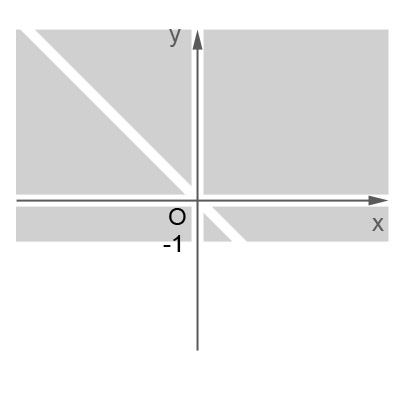
\includegraphics[width=0.4\textwidth]{Img1B.jpg}
  \end{center}
\end{figure}
% -  -  -  -  -  -  -  -  -  -  -  -  -  -  -  -  -  -  -  -  -  -  -  -  -  -  -  -  -  -  
% PART C
\item The function is not defined when the denominator is zero, so we require that $x^2+y^2\ne1$. The domain can therefore be expressed as $D=\{(x,y)| x^2+y^2 \ne 1 \}$. The numerator can take on any value, so the function $f$ can take on any value, so the range is $\mathbb{R}$.
\begin{figure}[!htbp]
  \begin{center}
    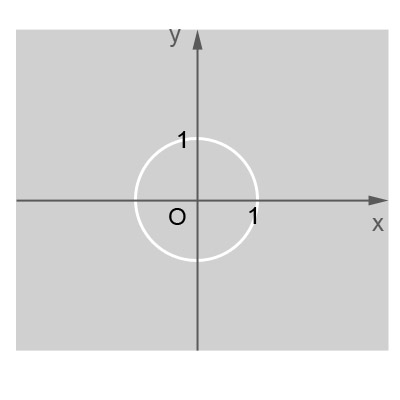
\includegraphics[width=0.4\textwidth]{Img1C.jpg}
  \end{center}
\end{figure}
% -  -  -  -  -  -  -  -  -  -  -  -  -  -  -  -  -  -  -  -  -  -  -  -  -  -  -  -  -  -  
% PART D
\newpage
\item For the domain, we require that 
\begin{align*}
x+2y &> 0  \text{, or } y > - x/2.
\end{align*}
The domain can therefore be expressed as $D=\{(x,y)|y > - x/2\}$. The function $f$ can take on any value, so the range is $\mathbb{R}$.
\begin{figure}[!htbp]
  \begin{center}
    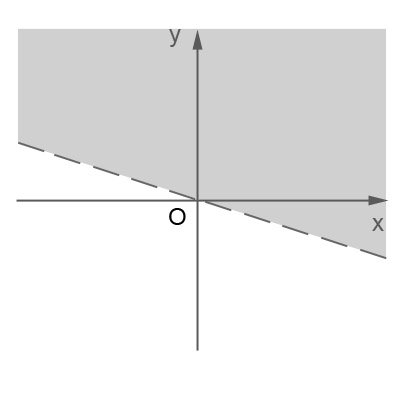
\includegraphics[width=0.4\textwidth]{Img1D.jpg}
  \end{center}
\end{figure}
% -  -  -  -  -  -  -  -  -  -  -  -  -  -  -  -  -  -  -  -  -  -  -  -  -  -  -  -  -  -  
\end{enumerate}

% ~~~~~~~~~~~~~~~~~~~~~~~~~~~~~~~~~~~~~~~~~~~~~~~~~~~~~~~~~
\item
% LIMIT SOLUTIONS
% -  -  -  -  -  -  -  -  -  -  -  -  -  -  -  -  -  -  -  -  -  -  -  -  -  -  -  -  -  -  
\begin{enumerate}
\item We can simply evaluate the limit to obtain
\begin{align*}
\lim_{(r,s)\rightarrow(0,2\pi) } \frac{3r^2+rs^3-3\sin (s/4)}{r^2}
&= \lim_{(r,s)\rightarrow(0,2\pi) }3+\frac{s^3}{r}-3r^2\sin (s/4)
\end{align*}
Because of the $s^3/r$ term, this limit tends to infinity, and therefore does not exist.
% -  -  -  -  -  -  -  -  -  -  -  -  -  -  -  -  -  -  -  -  -  -  -  -  -  -  -  -  -  -  
\item Let $f(x,y) = (x-y)/(x+y)$. Along the $x$-axis, $f=f(x,0)$, so 
\begin{align*}
f(x,0) = \frac{x}{x} = 1, \quad x\ne 0.
\end{align*}
A similar calculation shows that along the $y$-axis, $f$ = -1, if $y\ne0$. If we approach the point $(0,0)$ along the $x$-axis and the $y$-axis, we find that 
\begin{align*}
\text{along the $x$-axis, } & f = f(x,0),\text{ and } f \rightarrow +1 \\
\text{along the $y$-axis, } & f = f(0,y),\text{ and } f \rightarrow -1 
\end{align*}
These limits are not equal, and so the limit does not exist. 
% -  -  -  -  -  -  -  -  -  -  -  -  -  -  -  -  -  -  -  -  -  -  -  -  -  -  -  -  -  -  
\item We can simply evaluate the limit to obtain 
\begin{align*}
  \lim_{(x,y,z)\rightarrow(1,1,1)} \big|3x - 2y - z \big| = 3 -2 -1 = 0
\end{align*}
% -  -  -  -  -  -  -  -  -  -  -  -  -  -  -  -  -  -  -  -  -  -  -  -  -  -  -  -  -  -  
\item  Let $f(x,y,z) = (x^2-y^2-z^2)/(x^2+y^2+z^2)$. Then, along the $x$-axis, $f=(x,0,0)$. As long as $x$ is not zero, $f$ is equal to 1. However, along the $y$-axis, $f=f(0,y,0)$. Provided that $y$ is not zero, $f$ is equal to -1. Therefore,
\begin{align*}
\text{along the $x$-axis, } & f \rightarrow +1 \\
\text{along the $y$-axis, } & f \rightarrow -1 
\end{align*}
These limits are not equal, and so the limit does not exist. 
% -  -  -  -  -  -  -  -  -  -  -  -  -  -  -  -  -  -  -  -  -  -  -  -  -  -  -  -  -  -  
\item  We can evaluate this limit by rationalizing the numerator.
\begin{align*}
  \lim_{(x,y)\rightarrow(1,0) } \frac{\sqrt{2x+y}-\sqrt{2x-y}}{2y} &= 
  \lim_{(x,y)\rightarrow(1,0) } \frac{\sqrt{2x+y}-\sqrt{2x-y}}{2y} \Bigg(\frac{\sqrt{2x+y}+\sqrt{2x-y}}{\sqrt{2x+y}+\sqrt{2x-y}} \Bigg) \\
  &=\lim_{(x,y)\rightarrow(1,0) } \frac{(2x+y)-(2x-y)}{2y \Big(\sqrt{2x+y}+\sqrt{2x-y} \Big)}  \\
  &=\lim_{(x,y)\rightarrow(1,0) } \frac{2y}{2y \Big(\sqrt{2x+y}+\sqrt{2x-y} \Big)}  \\
  &=\lim_{(x,y)\rightarrow(1,0) } \frac{1}{\sqrt{2x+y}+\sqrt{2x-y} }  \\
  &= \frac{1}{2\sqrt{2} }\\
  &= \frac{\sqrt{2}}{2}
\end{align*}
% -  -  -  -  -  -  -  -  -  -  -  -  -  -  -  -  -  -  -  -  -  -  -  -  -  -  -  -  -  -  
\end{enumerate}
% ~~~~~~~~~~~~~~~~~~~~~~~~~~~~~~~~~~~~~~~~~~~~~~~~~~~~~~~~~
\item
% CONTINUITY 
The given function is defined everywhere. Now, for it to be continuous at any point $(x_0,y_0,z_0)$, we require that 
\begin{align*} 
   \lim_{(x,y,z)\rightarrow(x_0,y_0,z_0) } g(x,y,z) = g(x_0,y_0,z_0)
 \end{align*}
If we evaluate the limit as $g$ approaches $(0,0,1)$, we have
\begin{align*}
\lim_{(x,y,z)\rightarrow(0,0,1) } f(x,y,z) 
&= \lim_{(x,y,z)\rightarrow(0,0,1) } x+y+2z \\
&= 0+0+2(1) \\
&= 2
\end{align*}
However, at $(0,0,1)$, $g = 2$. So the given function is not continuous at the point $(0,0,1)$. Elsewhere, the function is a polynomial in three variables, and so will be continuous everywhere except at the point $(0,0,1)$. 
% ~~~~~~~~~~~~~~~~~~~~~~~~~~~~~~~~~~~~~~~~~~~~~~~~~~~~~~~~~
\item The lines $y=m(x-1)$ all pass through the limit point, $(1,0)$, where $m$ is any real number. Approaching the limit point along these lines, our limit becomes
\begin{align*} 
   \lim_{(x,y)\rightarrow(1,0) } \frac{x(x-1)^3 + y^2}{4(x-1)^2+9y^3} 
   &= \lim_{(x,y)\rightarrow(1,0) } \frac{x(x-1)^3 + m^2(x-1)^2}{4(x-1)^2+9m^3(x-1)^3} \\
   &= \lim_{(x,y)\rightarrow(1,0) } \frac{x(x-1) + m^2}{4+9(x-1)} \\
   &= \frac{m^2}{4}
 \end{align*}
 The result depends on $m$, which is an arbitrary value. Therefore, the limit does not exist. 
% ~~~~~~~~~~~~~~~~~~~~~~~~~~~~~~~~~~~~~~~~~~~~~~~~~~~~~~~~~

\item
\begin{enumerate}
\item To plot the level curves, we set $z = c$, and solve for $y$: 
\begin{align*} 
  c &= \frac{\ln y}{x^2} \\
  cx^2&= \ln y \\
  y &= e^{cx^2}
\end{align*}
\begin{figure}[!htbp]
  \begin{center}
    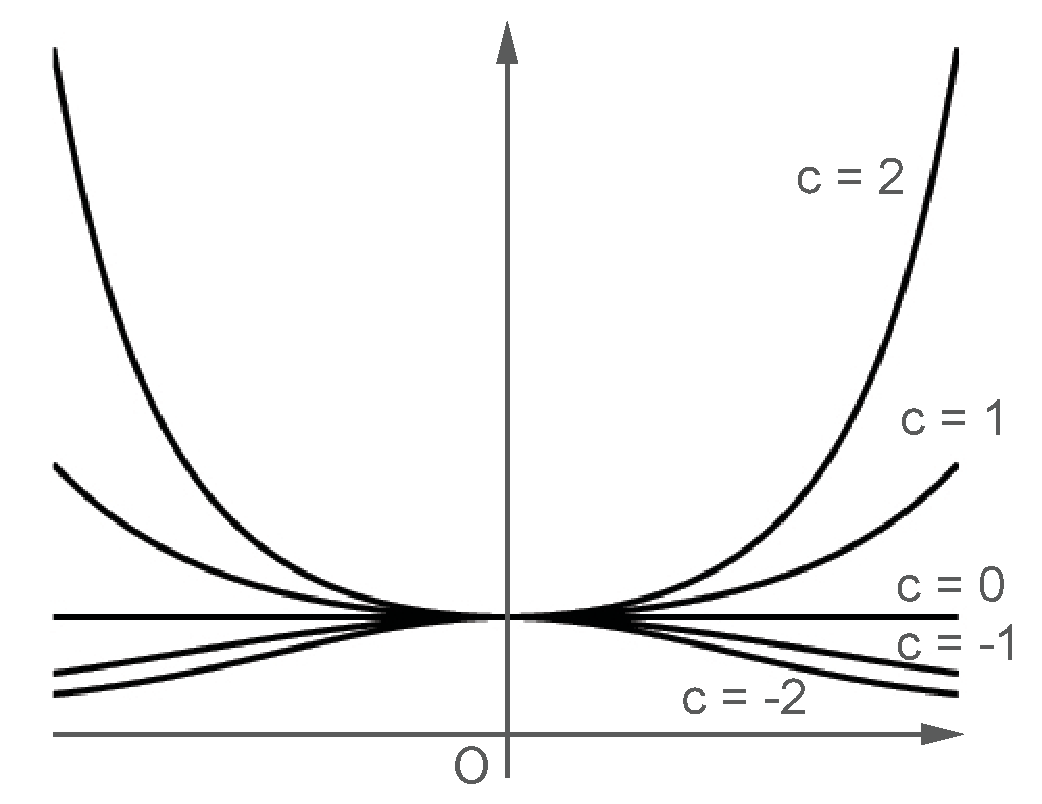
\includegraphics[width=0.4\textwidth]{ImgLevelCurvesA.pdf}
  \end{center}
\end{figure}
% -  -  -  -  -  -  -  -  -  -  -  -  -  -  -  -  -  -  -  -  -  -  -  -  -  -  -  -  -  -  
\item To plot the level curves, we set $z = c$, and solve for $y$: 
\begin{align*} 
  c &= \frac{x^2}{x^2+y^2} \\
  cy^2 &= (1-c)x^2
\end{align*}
If $c=0$, then we obtain the level curve $x = 0$. If $c \ne0$, then
\begin{align*} 
  y &= \pm \sqrt{\frac{1-c}{c}}x, \quad c \ne0
\end{align*}
For $c=2$, $y$ is undefined, so the level curves do not exist. The level curves for the other values of $c$ are shown in the graph below and are as follows:
\begin{align*} 
  \text{if } c&=0, \quad x = 0 \text{ (the vertical line that lies on the } y \text{-axis})\\
  \text{if } c&=1/4, y = \pm \sqrt{3}x\\
  \text{if } c&=1/2, y = \pm x\\  
  \text{if } c&=1, \quad y = 0    
\end{align*}

\begin{figure}[!htbp]
  \begin{center}
    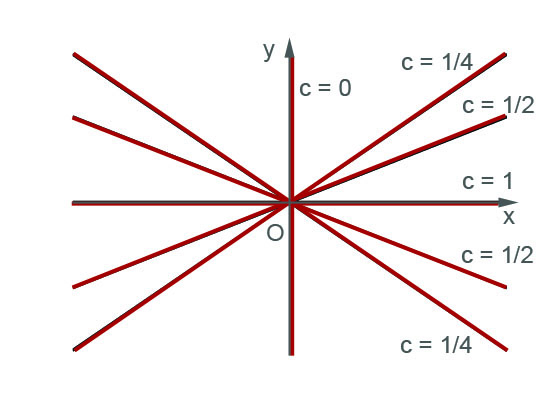
\includegraphics[width=0.4\textwidth]{ImgLevelCurvesB.jpg}
  \end{center}
\end{figure}

\end{enumerate}
% ~~~~~~~~~~~~~~~~~~~~~~~~~~~~~~~~~~~~~~~~~~~~~~~~~~~~~~~~~
\item
\begin{enumerate}
\item The set of straight lines that pass through $(2,1)$ are given by $y = c(x-2) + 1$. Rearranging yields the equation 
\begin{align*}
c = \frac{y-1}{x-2}
\end{align*}
The desired function is 
\begin{align*}
f(x,y) = \frac{y-1}{x-2}
\end{align*}
\item The set of circles with radius $e^c$ are given by $x^2 + y^2 = e^c$. Applying the natural logarithm to both sides of the equation yields 
\begin{align*}
\ln(x^2+y^2) = c
\end{align*}
The desired function is 
\begin{align*}
f(x,y) =\ln(x^2+y^2)
\end{align*}\end{enumerate}
% ~~~~~~~~~~~~~~~~~~~~~~~~~~~~~~~~~~~~~~~~~~~~~~~~~~~~~~~~~
% PROVIDE EXAMPLE, LIMIT
\item 
\begin{enumerate}
\item
Suppose we let 
\begin{align*}
f(x,y) = \frac{y}{(x-1)^2}
\end{align*}
Then, along any parabola $y = m(x-1)^2$ the limit becomes
\begin{align*}
\lim_{(x,y)\rightarrow(1,0) } \frac{y}{(x-1)^2} = \lim_{(x,y)\rightarrow(1,0) } \frac{m(x-1)^2}{(x-1)^2} = m
\end{align*}
The function we chose therefore meets the specified criteria.
\item
The limit cannot exist because the limit depends on $m$, which is an arbitrary real number.
\end{enumerate}
% ~~~~~~~~~~~~~~~~~~~~~~~~~~~~~~~~~~~~~~~~~~~~~~~~~~~~~~~~~
% TEMPERATURE DISTRIBUTION
\item 
\BEN
\item The temperature can be written as 
\begin{align*}T(x,y) = \frac{k}{\sqrt{x^2 + y^2}},\end{align*} 
where $k$ is an unknown constant of proportionality.
\item The level curves are solution sets of the equation $T(x,y)=c$, for $c\in\R$. Therefore,
\begin{align*}
  T(x,y) = c &= \frac{k}{\sqrt{x^2 + y^2}} \\
  c^2 &= \frac{k^2}{x^2 + y^2} \\
  x^2 + y^2 &= \frac{k^2}{c^2}
\end{align*} 
The level curves are concentric circles with radius $k/c$. 
\item At the point (2,1), the temperature is known, which allows us to solve for $k$. 
\begin{align*}
  T(2,1) = 10 &= \frac{k}{\sqrt{2^2 + 1^2}}\\
  k& = 10\sqrt{5}
\end{align*} 
At (1,3), the temperature is
\begin{align*}
  T(1,3) &= \frac{10\sqrt{5}}{\sqrt{1^2 + 3^2}}\\
  & = 10\sqrt{\frac{5}{4}}
\end{align*} 
\EEN
% ~~~~~~~~~~~~~~~~~~~~~~~~~~~~~~~~~~~~~~~~~~~~~~~~~~~~~~~~~
% ELECTRIC POTENTIAL DISTRIBUTION
\item The level curves are solution sets of the equation $V(x,y) = K$, for constant $K\in\R$.
\begin{align*}
V(x,y) = K &= \frac{c}{\sqrt{r^2 - x^2 -y^2}} \\
r^2-x^2-y^2 &= \frac{c^2}{K^2} \\
x^2+y^2 &= r^2 -  \frac{c^2}{K^2}
\end{align*}
The left-hand side must be positive, so we must have that 
\begin{align*}
r^2 &>  \frac{c^2}{K^2}\\
K^2 &> c^2/r^2\\
 |K| &<  |c|/|r|
\end{align*}
But $c, K$, and $r$ are all positive constants, so this simplifies to $K<\frac{c}{r}$. The level curves are concentric circles, centered at the origin, with radius $r^2 -  \frac{c^2}{K^2}$, for $K<\frac{c}{r}$.
% ~~~~~~~~~~~~~~~~~~~~~~~~~~~~~~~~~~~~~~~~~~~~~~~~~~~~~~~~~
% LIMIT PROOF
\item 
If we approach the limit point along the $x$-axis, then $y=0$ and we obtain
\begin{align*}
  \lim_{(x,y)\rightarrow(0,0) } \frac{x(0)^2}{x^2+(0)^2} = 0
\end{align*}
We obtain the same result if we approach the origin along the $y$-axis, or along any line $y=mx$. It would seem that the limiting value could exist and could be equal to 0. To show that this is the case, we must show that for any $\epsilon > 0$, there exists a $\delta > 0$ such that   
\begin{align*}
 \Big|  \frac{xy^2}{x^2+y^2} - 0 \Big| < \epsilon \text{  whenever  } 0 < \sqrt{(x-0)^2 + (y-0)^2} < \delta ,
\end{align*}
or simply
\begin{align*}
 \Big|  \frac{xy^2}{x^2+y^2} \Big| < \epsilon \text{  whenever  } 0 < \sqrt{x^2 + y^2} < \delta .
\end{align*}
Now, $\big| x^2 + y^2\big| = x^2 + y^2$, and $|y^2| = y^2$, so
\begin{align*}
 \Big|  \frac{xy^2}{x^2+y^2} \Big| &=  \frac{ \big|xy^2 \big|}{ \big|x^2+y^2 \big|}  =   \frac{ \big|x\big|y^2 }{ x^2+y^2 }
\end{align*}
Also, $|x| \le \sqrt{x^2+y^2}$, and $y^2 \le x^2+y^2$, so
\begin{align*}
 \Big|  \frac{xy^2}{x^2+y^2} \Big| 
 &=  \frac{ \big|x\big|y^2 }{ x^2+y^2 }\\
 &\le \frac{ \ \sqrt{x^2+y^2} ( x^2+y^2 ) }{ x^2+y^2 }\\
 &= \sqrt{x^2+y^2}
\end{align*}
So if $\delta = \epsilon$, then 
\begin{align*}
 \Big|  \frac{xy^2}{x^2+y^2} \Big| < \epsilon \text{  whenever  } 0 < \sqrt{x^2 + y^2} < \delta .
\end{align*}
% ~~~~~~~~~~~~~~~~~~~~~~~~~~~~~~~~~~~~~~~~~~~~~~~~~~~~~~~~~

\EEN
